\documentclass[a4paper]{article}
% mathematische symbolen
\usepackage{geometry}
\geometry{verbose,a4paper,tmargin=2.5cm,bmargin=2.5cm,lmargin=2.5cm,rmargin=2.5cm}
\usepackage[dutch]{babel}
\usepackage{float}
\usepackage{hyperref}
\usepackage{graphicx}
\usepackage{caption}
\usepackage{subcaption}
\usepackage{tabularx}
\usepackage{booktabs}
\usepackage{amssymb}
\usepackage{amsmath,amsthm}
\usepackage{commath}
\usepackage{latexsym}
\usepackage{amsfonts}
\usepackage{mathrsfs}
\usepackage{listings}
\usepackage{parskip}
\renewcommand{\qedsymbol}{QED}
\theoremstyle{plain} %gebruikelijke stijl voor beweringen e.d.
\newtheorem*{vermoeden}{Vermoeden}
\newtheorem*{stelling}{Stelling}
\newtheorem*{bewering}{Bewering}
\theoremstyle{definition} %gebruikelijke stijl voor definities e.d.
\newtheorem*{definitie}{Definitie}
\newtheorem*{tegenvoorbeeld}{Tegenvoorbeeld}
\title{IN4086-14  Data Visualization: Visual Game Analytics} %vul "Herkansing" in als je een herkansing inlevert
\author{Vikko Smit\\ %nieuwe regel voor deze auteur
1293478
\and
Bastiaan Gris\`el\\
4090438
}
\begin{document}
\maketitle %produceert de daadwerkelijke titelinformatie

\section*{Introduction}
This assignment is about analyzing data from many matches of DOTA2, a MOBA-style computer game that went up to an impressive 8 million players worldwide last summer. 
The game is played in two teams of five players (heroes) and the team that first destroys the other team's base building (ancient) wins. 
The game also involves pushing waves of computer controlled players (NPCs) to three lanes while enemy players try to push the waves of NPCs your way. 
A reward is obtained for killing each enemy NPC or team member in the form of gold and experience (which makes the player grow in strength).

A key aspect is this game is positioning on the playing field. 
A player might want to stay close to battling NPCs to get their gold and experience. 
Of course, each team will try to gain experience themselves and block the enemy players from getting it. 
In order to achieve good results, teamplay is very important as teammates can help to eliminate an enemy or get an advantage against NPCs.

\section*{Problem setting}
Our focus is to make a game visualization to help people that review and comment on DOTA games to identify important moves and global activity of players. 
We want to achieve this by giving every player a trail of his last position and a smart detector that identifies threats in the neighborhood and notifies you where important actions are likely to be made.

A first challenge is that there is a lot of data to be loaded and processed, this causes many systems to crash if used in one chunk. 
However, we don't want to limit ourselves to a small subset of the data since one might select matches that are not very interesting to see.
To make the data handling more robust to larger volumes we imported and indexed all locations of the players of all matches in a small mongoDB database. 
With this solution all data is still available and can be retrieved very fast in a web request.

In order to get a good overview of the game, players have to be drawn on a top-view map of the game.
Since the dimensions of the map differs per browser / resolution setting, we chose for a solution with a grid mapped to the picture where you could enter player coordinates from the database that are instantly converted to a drawing of a dot on the respective coordinate with the respective team color. 

\section*{Solution}
The solutions consists of two different parts, each solving a different part of the problem.

\subsection*{Trail of movement}
The trail of movement is based on quite a simple idea:  draw a line with a fixed $\delta$t of all the positions you have been until the current time stamp. By including this data in the visualization, it is clear how players move instead of seeing them on one point in time. It also gives an idea of the speed with which players are moving, since distance over time is their speed (so a longer trail means a higher speed). These trails make for a great analysis tool and can even help to predict an player's next action.

\subsection*{Proximity detection}
In order to detect important moves and overall points of interest, we have chosen to focus on the players that are in danger. We have thought of a model that can quantify this danger and detect battles between players.

The algorithm is based on the absolute distance from every player to every ally and every enemy, from now on called $d_{a,i}$ as the distance to ally $a_i$ and $d_{e,i}$ as a distance to enemy $e_i$. A player is in more danger when there are enemies around it and in less danger when there are a lot of allies nearby. To account for this, the data is normalized according to $D_{a,i} = 1- \frac{d_{a,i}}{radius}$ and $D_{a,i} = 1- \frac{d_{e,i}}{radius}$, which indicates if another player is within a certain \emph{radius}. We only look at the value of $D_{a,i}$ and $D_{e,i}$ that lie within the $[0,1]$ region, 0 meaning that another player is just in range and 1 meaning that another player is practically on top of the player while values that are below 0 mean that the other player is too far away to count as dangerous.

The value of $D_{a,i}$ can also be transformed with for instance a square root, so the players that are very close (in range of attacking) all have a more-or-less equal danger level. To quantify danger, the sum of all distances to the enemy can be subtracted form the distances to the allies, ending up with a high value if enemies are closer to you in relation to your friends and a battle of this outnumbered player might soon be happening.

There is another thing that needs to be accounted for, namely you always have 1 ally close, which is yourself. The sum of all the distances to other players  within a \emph{radius} can be $[0,1,2,3,4,5]$ for the enemy and only $[1,2,3,4,5]$ for the allies. The difference between enemies and allies nearby can take on a range of $[-5,4]$. The equilibrium in this range lies at -0.5. To get it nicely at 0 while still having a linear scale from -5 (theoretical minimum danger) to +5 (theoretical maximum danger) we apply the following formula:

$Danger(player) = \frac{5}{4.5}(\sum_i{\sqrt{D_{e,i}}}-\sum_i{\sqrt{D_{a,i}}}+\frac{1}{2})$\\

This value can be used to draw bar charts of how dangerous people are positioned at the moment in respect to the other players, but when given a arbitrarily chosen threshold this would also point out Points of Interest for the reviewer to pay some attention to. Our points of interest are players that exceed a certain threshold of positive danger. 

When multiple players are within the radius of the proximity detector and have a high danger value (for instance when 3 players stick together, but get attacked by 5 players of the other team) then the players are clustered to a average coordinate of the players in danger. This new virtual 'player' is then displayed as the point of interest instead of the player's individual coordinates.

\newpage

\section*{Results}
When we tested the visualization on one of the test matches (match: 569649581, time: 199, history:10 steps) we found a nice example on how these visualizations are working to their optimal. Lines give a clear indication of what just happened and what the direction and speed of the players is, while the proximity detector places circles around points that you might want to watch.
\begin{figure}[h!]
 	\centering
    	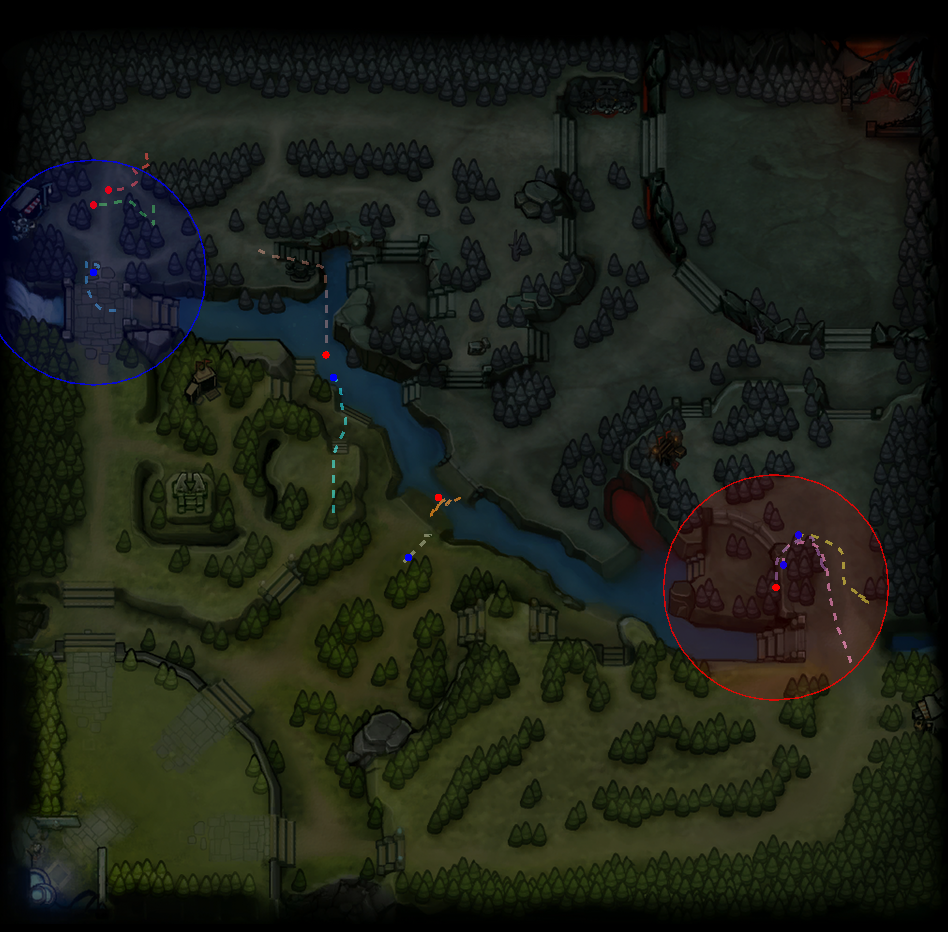
\includegraphics[width=0.5\textwidth]{proximity}
\caption*{Points of interest and trails of movement}
\end{figure}

In this picture you can see the blue player in the top left being pressured in a 2 versus 1 standoff, while in the bottom right a red player is being chased by two opponents and is trying to get away.

Watching a few plays we haven't seen much clustering happening, but maybe if you switch to Pro games, where more teamwork is involved and people are more likely to be outnumbered in a mass vs mass battle.

The application database had a size of around 4GB, it was a little hard to send over the email. We have therefore decided to host a demo at \url{http://datavis.vikko.nl}.
\end{document}